\documentclass[tikz,border=8pt]{standalone}
\usepackage[dvipsnames]{xcolor}
\usetikzlibrary{shapes.geometric,arrows.meta,positioning,fit,backgrounds,calc}

\begin{document}
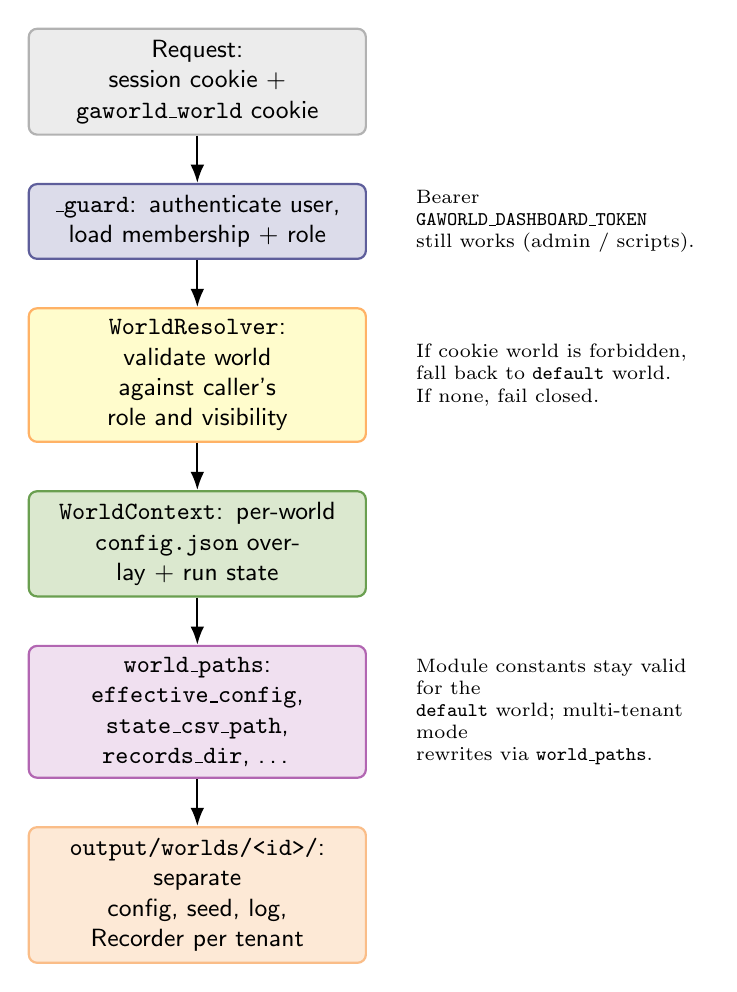
\begin{tikzpicture}[
  font=\sffamily\small,
  layer/.style={rectangle, draw, thick, rounded corners=3pt, align=center, minimum height=0.8cm, inner sep=4pt},
  req/.style={layer, fill=gray!15, draw=gray!60, text width=4.0cm},
  cookie/.style={layer, fill=yellow!20, draw=orange!60, text width=4.0cm},
  guard/.style={layer, fill=MidnightBlue!15, draw=MidnightBlue!70, text width=4.0cm},
  world/.style={layer, fill=OliveGreen!15, draw=OliveGreen!70, text width=4.0cm},
  paths/.style={layer, fill=Purple!12, draw=Purple!60, text width=4.0cm},
  fs/.style={layer, fill=Apricot!25, draw=Apricot!80, text width=4.0cm},
  ar/.style={-Latex, thick},
  >={Stealth[length=2.5mm]}
]

% Vertical flow
\node[req] (r1) at (0,0) {%
  Request:\\
  session cookie + \texttt{gaworld\_world} cookie};
\node[guard, below=0.6cm of r1] (g1) {%
  \texttt{\_guard}: authenticate user,\\
  load membership + role};
\node[cookie, below=0.6cm of g1] (c1) {%
  \texttt{WorldResolver}: validate world\\
  against caller's role and visibility};
\node[world, below=0.6cm of c1] (w1) {%
  \texttt{WorldContext}: per-world\\
  \texttt{config.json} overlay + run state};
\node[paths, below=0.6cm of w1] (p1) {%
  \texttt{world\_paths}: \texttt{effective\_config},\\
  \texttt{state\_csv\_path}, \texttt{records\_dir}, \ldots};
\node[fs, below=0.6cm of p1] (f1) {%
  \texttt{output/worlds/<id>/}: separate\\
  config, seed, log, Recorder per tenant};

% Arrows
\draw[ar] (r1) -- (g1);
\draw[ar] (g1) -- (c1);
\draw[ar] (c1) -- (w1);
\draw[ar] (w1) -- (p1);
\draw[ar] (p1) -- (f1);

% Side notes
\node[right=0.5cm of g1, font=\scriptsize, text width=3.6cm, align=left] {%
  Bearer \texttt{GAWORLD\_DASHBOARD\_TOKEN}\\
  still works (admin / scripts).};
\node[right=0.5cm of c1, font=\scriptsize, text width=3.6cm, align=left] {%
  If cookie world is forbidden,\\
  fall back to \texttt{default} world.\\
  If none, fail closed.};
\node[right=0.5cm of p1, font=\scriptsize, text width=3.6cm, align=left] {%
  Module constants stay valid for the\\
  \texttt{default} world; multi-tenant mode\\
  rewrites via \texttt{world\_paths}.};

\end{tikzpicture}
\end{document}
